
Numbers were created to represent different quantities of things with similar properties: rocks, grains, logs, seeds, cattle etc.
%% TODO:(accacio) add figures to represent different quantities of things (apples, rocks, birds, etc)
%%
\begin{marginfigure}[30mm]
  \centering
  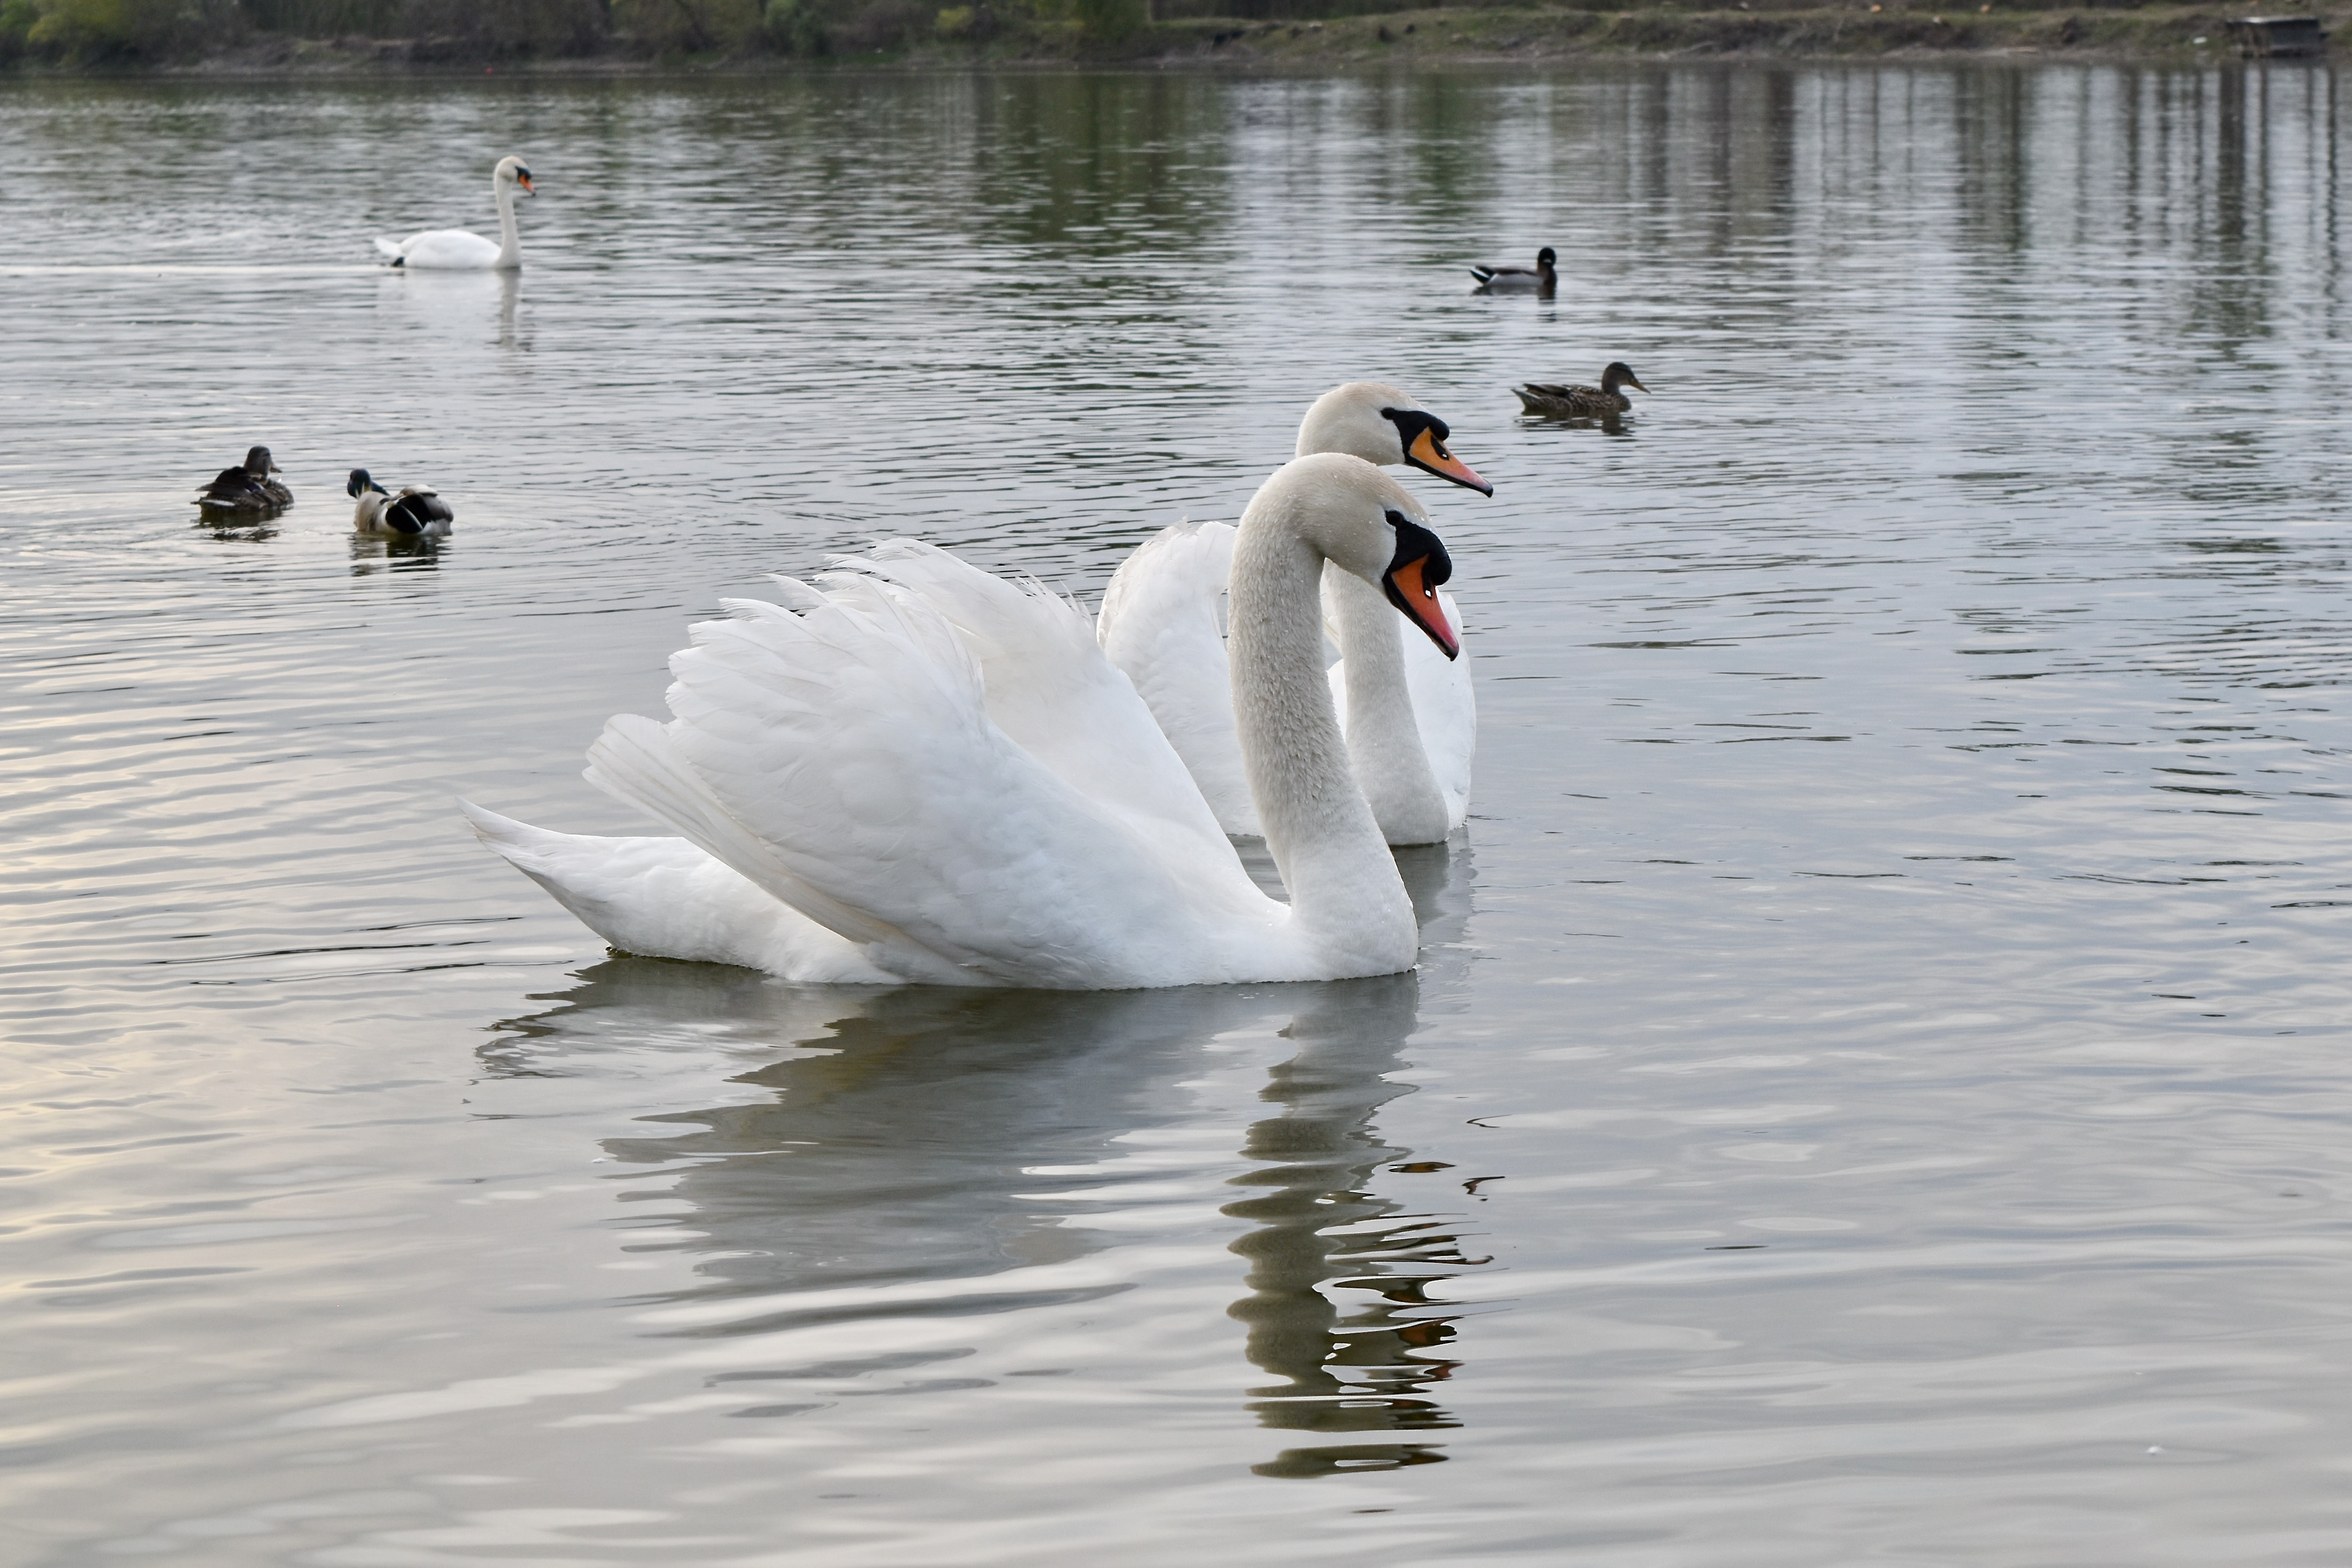
\includegraphics[width=\linewidth]{birds.jpeg}
  \caption[Birds swimming on the water.]{There are a different number of swans and ducks in this image.
    % 7 birds in this image, which 3 are swans and 4 are ducks.
  }\label{fig:birds}
\end{marginfigure}
Many numbering systems were created by different people, in different contexts, but they all share the counting purpose and have correspondent values.
Here are some examples:
\subsection{Hindu-Arabic numbers}
\[
  {1}\;
  {2}\;
  {3}\;
  {4}\;
  {5}\;
  {6}\;
  {7}\;
  {8}\;
  {9}
\]
\[
  {10}\;
  {20}\;
  {30}\;
  {40}\;
  {50}\;
  {60}\;
  {70}\;
  {80}\;
  {90}\;
  {100}
\]
\[
  {100}\;
  {200}\;
  {300}\;
  {400}\;
  {500}\;
  {600}\;
  {700}\;
  {800}\;
  {900}\;
  {1000}
\]
\subsection{Hieroglyphs}
\[
  \hg{1}\;
  \hg{2}\;
  \hg{3}\;
  \hg{4}\;
  \hg{5}\;
  \hg{6}\;
  \hg{7}\;
  \hg{8}\;
  \hg{9}
\]
\[
  \hg{10}\;
  \hg{20}\;
  \hg{30}\;
  \hg{40}\;
  \hg{50}\;
  \hg{60}\;
  \hg{70}\;
  \hg{80}\;
  \hg{90}\;
  \hg{100}
\]
\[
  \hg{100}\;
  \hg{200}\;
  \hg{300}\;
  \hg{400}\;
  \hg{500}\;
  \hg{600}\;
  \hg{700}\;
  \hg{800}\;
  \hg{900}\;
  \hg{1000}
\]

\subsection{Mayan numbers}
\[
  \maya{1}\;
  \maya{2}\;
  \maya{3}\;
  \maya{4}\;
  \maya{5}\;
  \maya{6}\;
  \maya{7}\;
  \maya{8}\;
  \maya{9}
\]
\[
  \maya{10}\;
  \maya{20}\;
  \maya{30}\;
  \maya{40}\;
  \maya{50}\;
  \maya{60}\;
  \maya{70}\;
  \maya{80}\;
  \maya{90}\;
  \maya{100}
\]
\[
  \maya{100}\;
  \maya{200}\;
  \maya{300}\;
  \maya{400}\;
  \maya{500}\;
  \maya{600}\;
  \maya{700}\;
  \maya{800}\;
  \maya{900}\;
  \maya{1000}
\]

\subsection{Roman numbers}
\[
  \rom{1}\;
  \rom{2}\;
  \rom{3}\;
  \rom{4}\;
  \rom{5}\;
  \rom{6}\;
  \rom{7}\;
  \rom{8}\;
  \rom{9}
\]
\[
  \rom{10}\;
  \rom{20}\;
  \rom{30}\;
  \rom{40}\;
  \rom{50}\;
  \rom{60}\;
  \rom{70}\;
  \rom{80}\;
  \rom{90}\;
  \rom{100}
\]
\[
  \rom{100}\;
  \rom{200}\;
  \rom{300}\;
  \rom{400}\;
  \rom{500}\;
  \rom{600}\;
  \rom{700}\;
  \rom{800}\;
  \rom{900}\;
  \rom{1000}
\]

Nowadays, great part of the world uses the Hindu-Arabic numeral system.

In Figure~\ref{fig:exampleNumbers} we can see the correspondence of some symbols of this number system with quantities of different objects.

\begin{figure}
  \centering
     \begin{subfigure}{.8\textwidth}
         \centering
         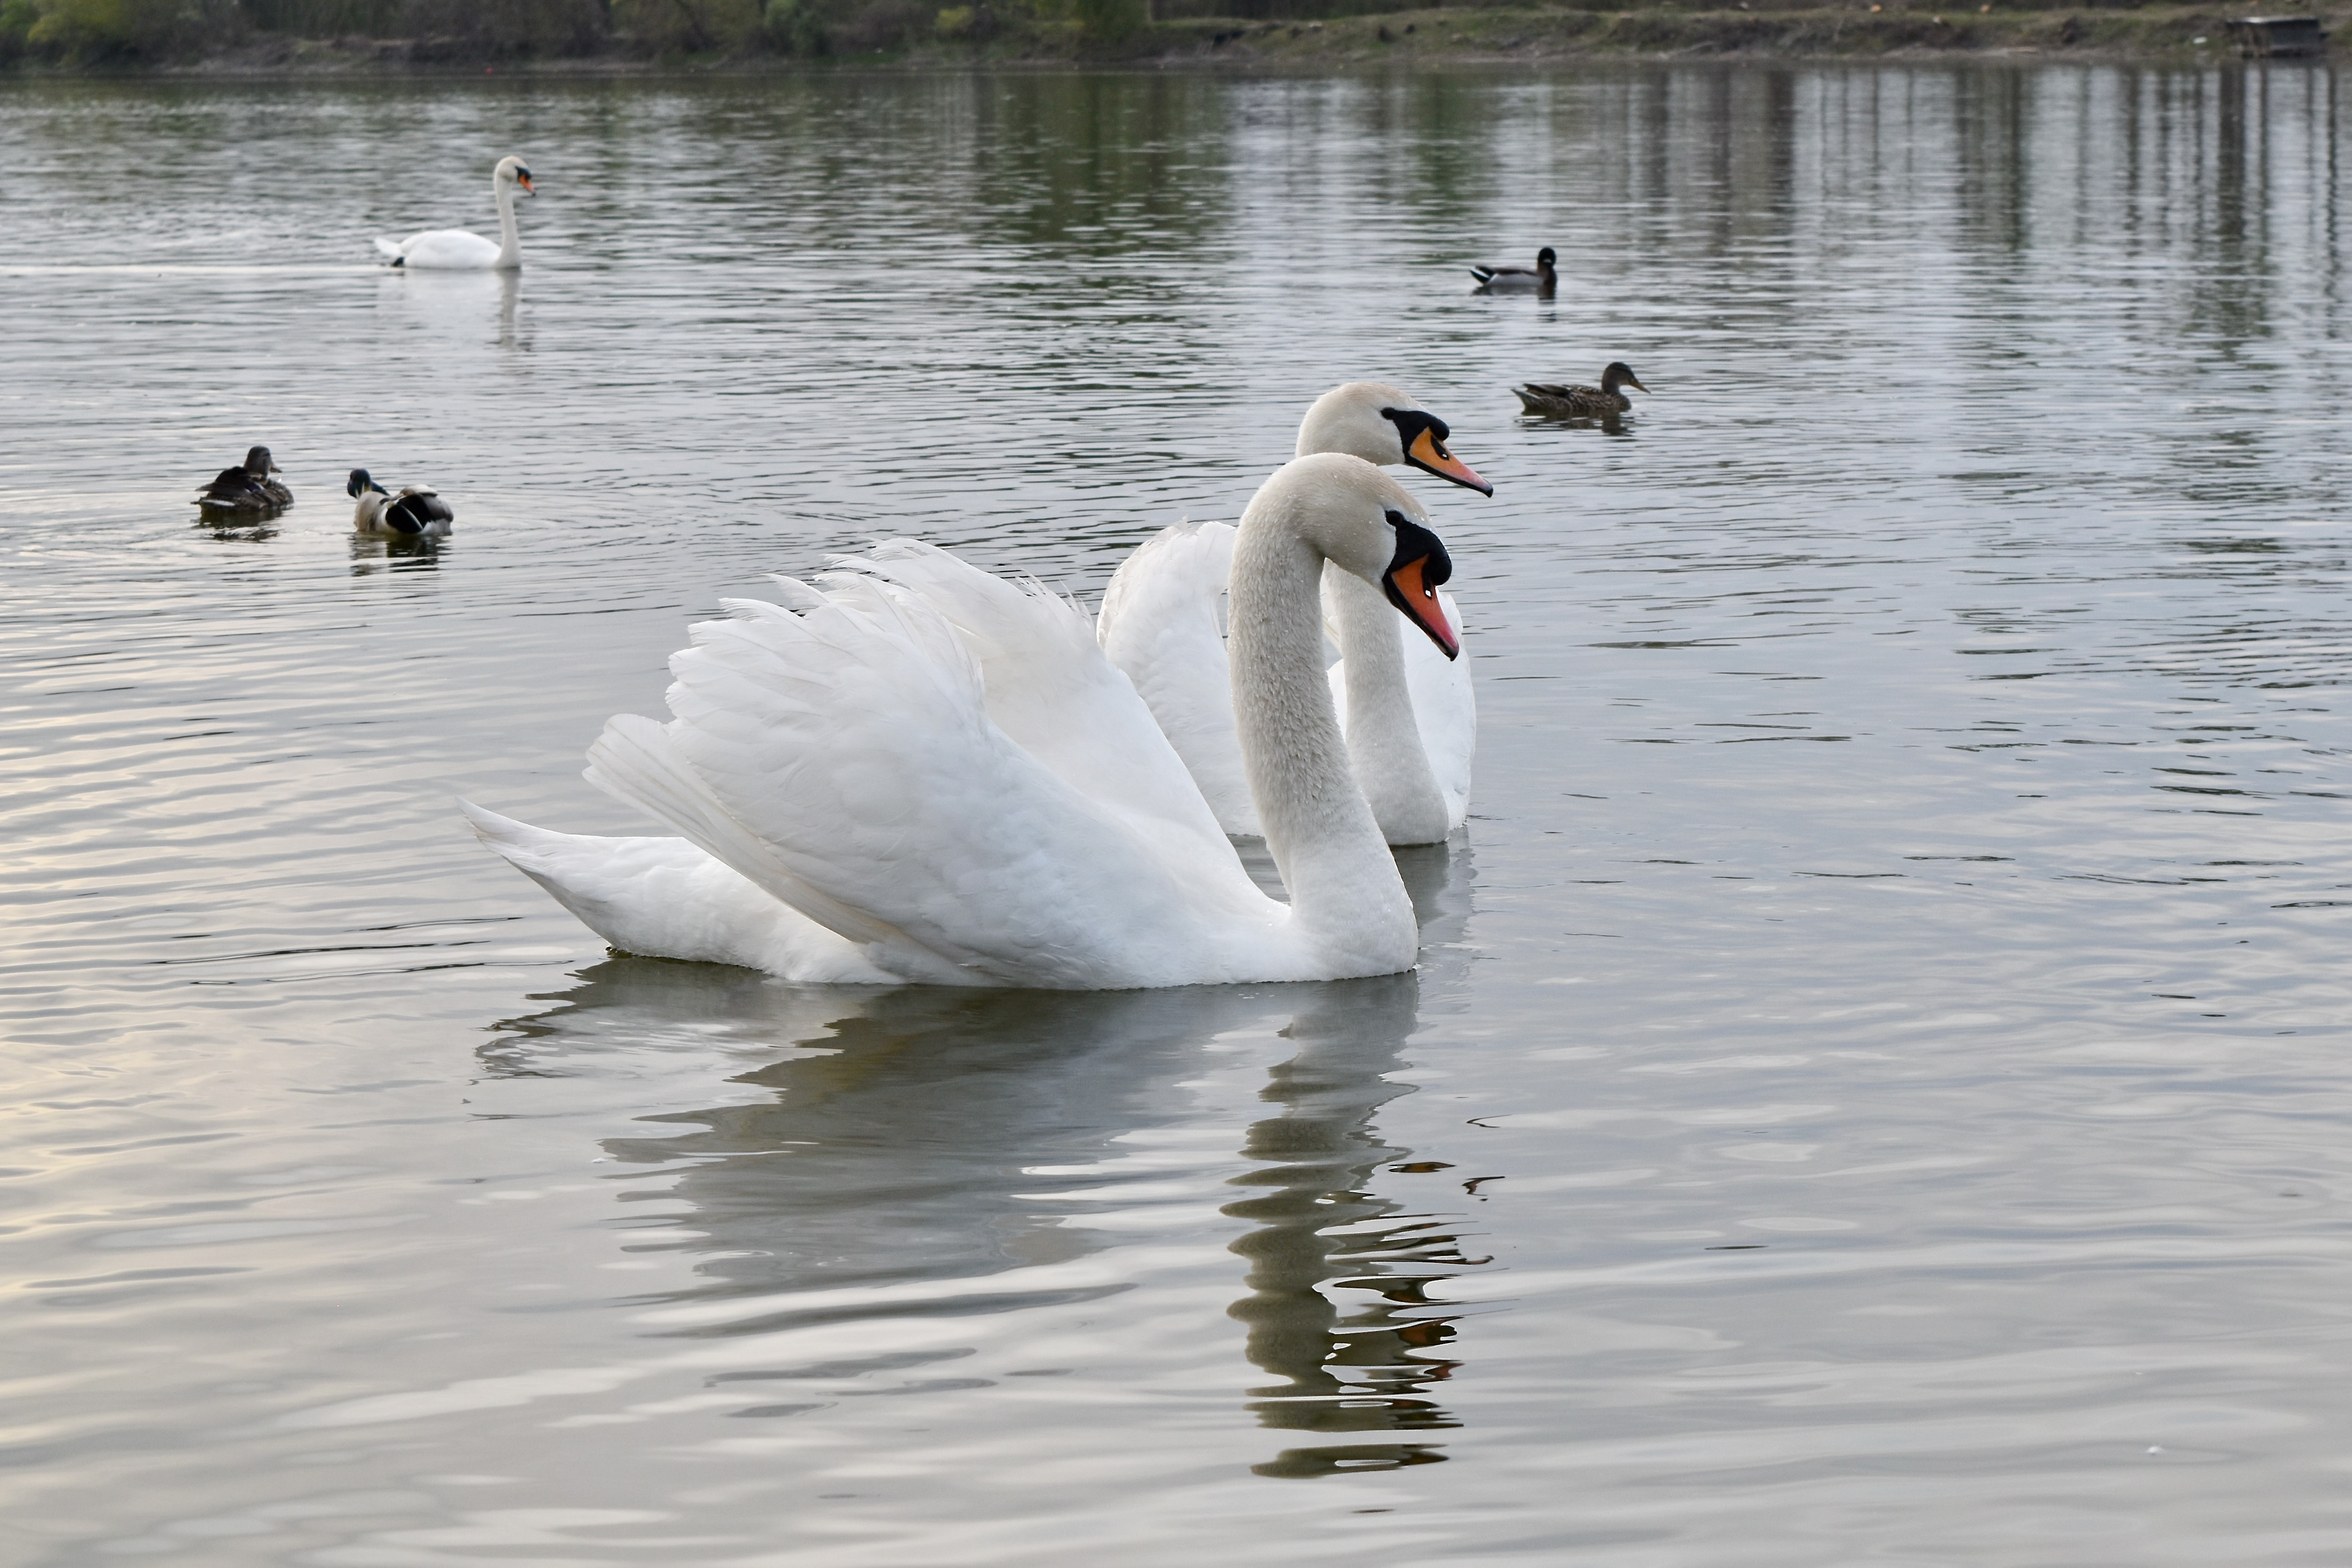
\includegraphics[width=\textwidth]{birds.jpeg}
         \caption{}
         \label{fig:birds}
     \end{subfigure}\\
     \begin{subfigure}{0.45\textwidth}
         \centering
         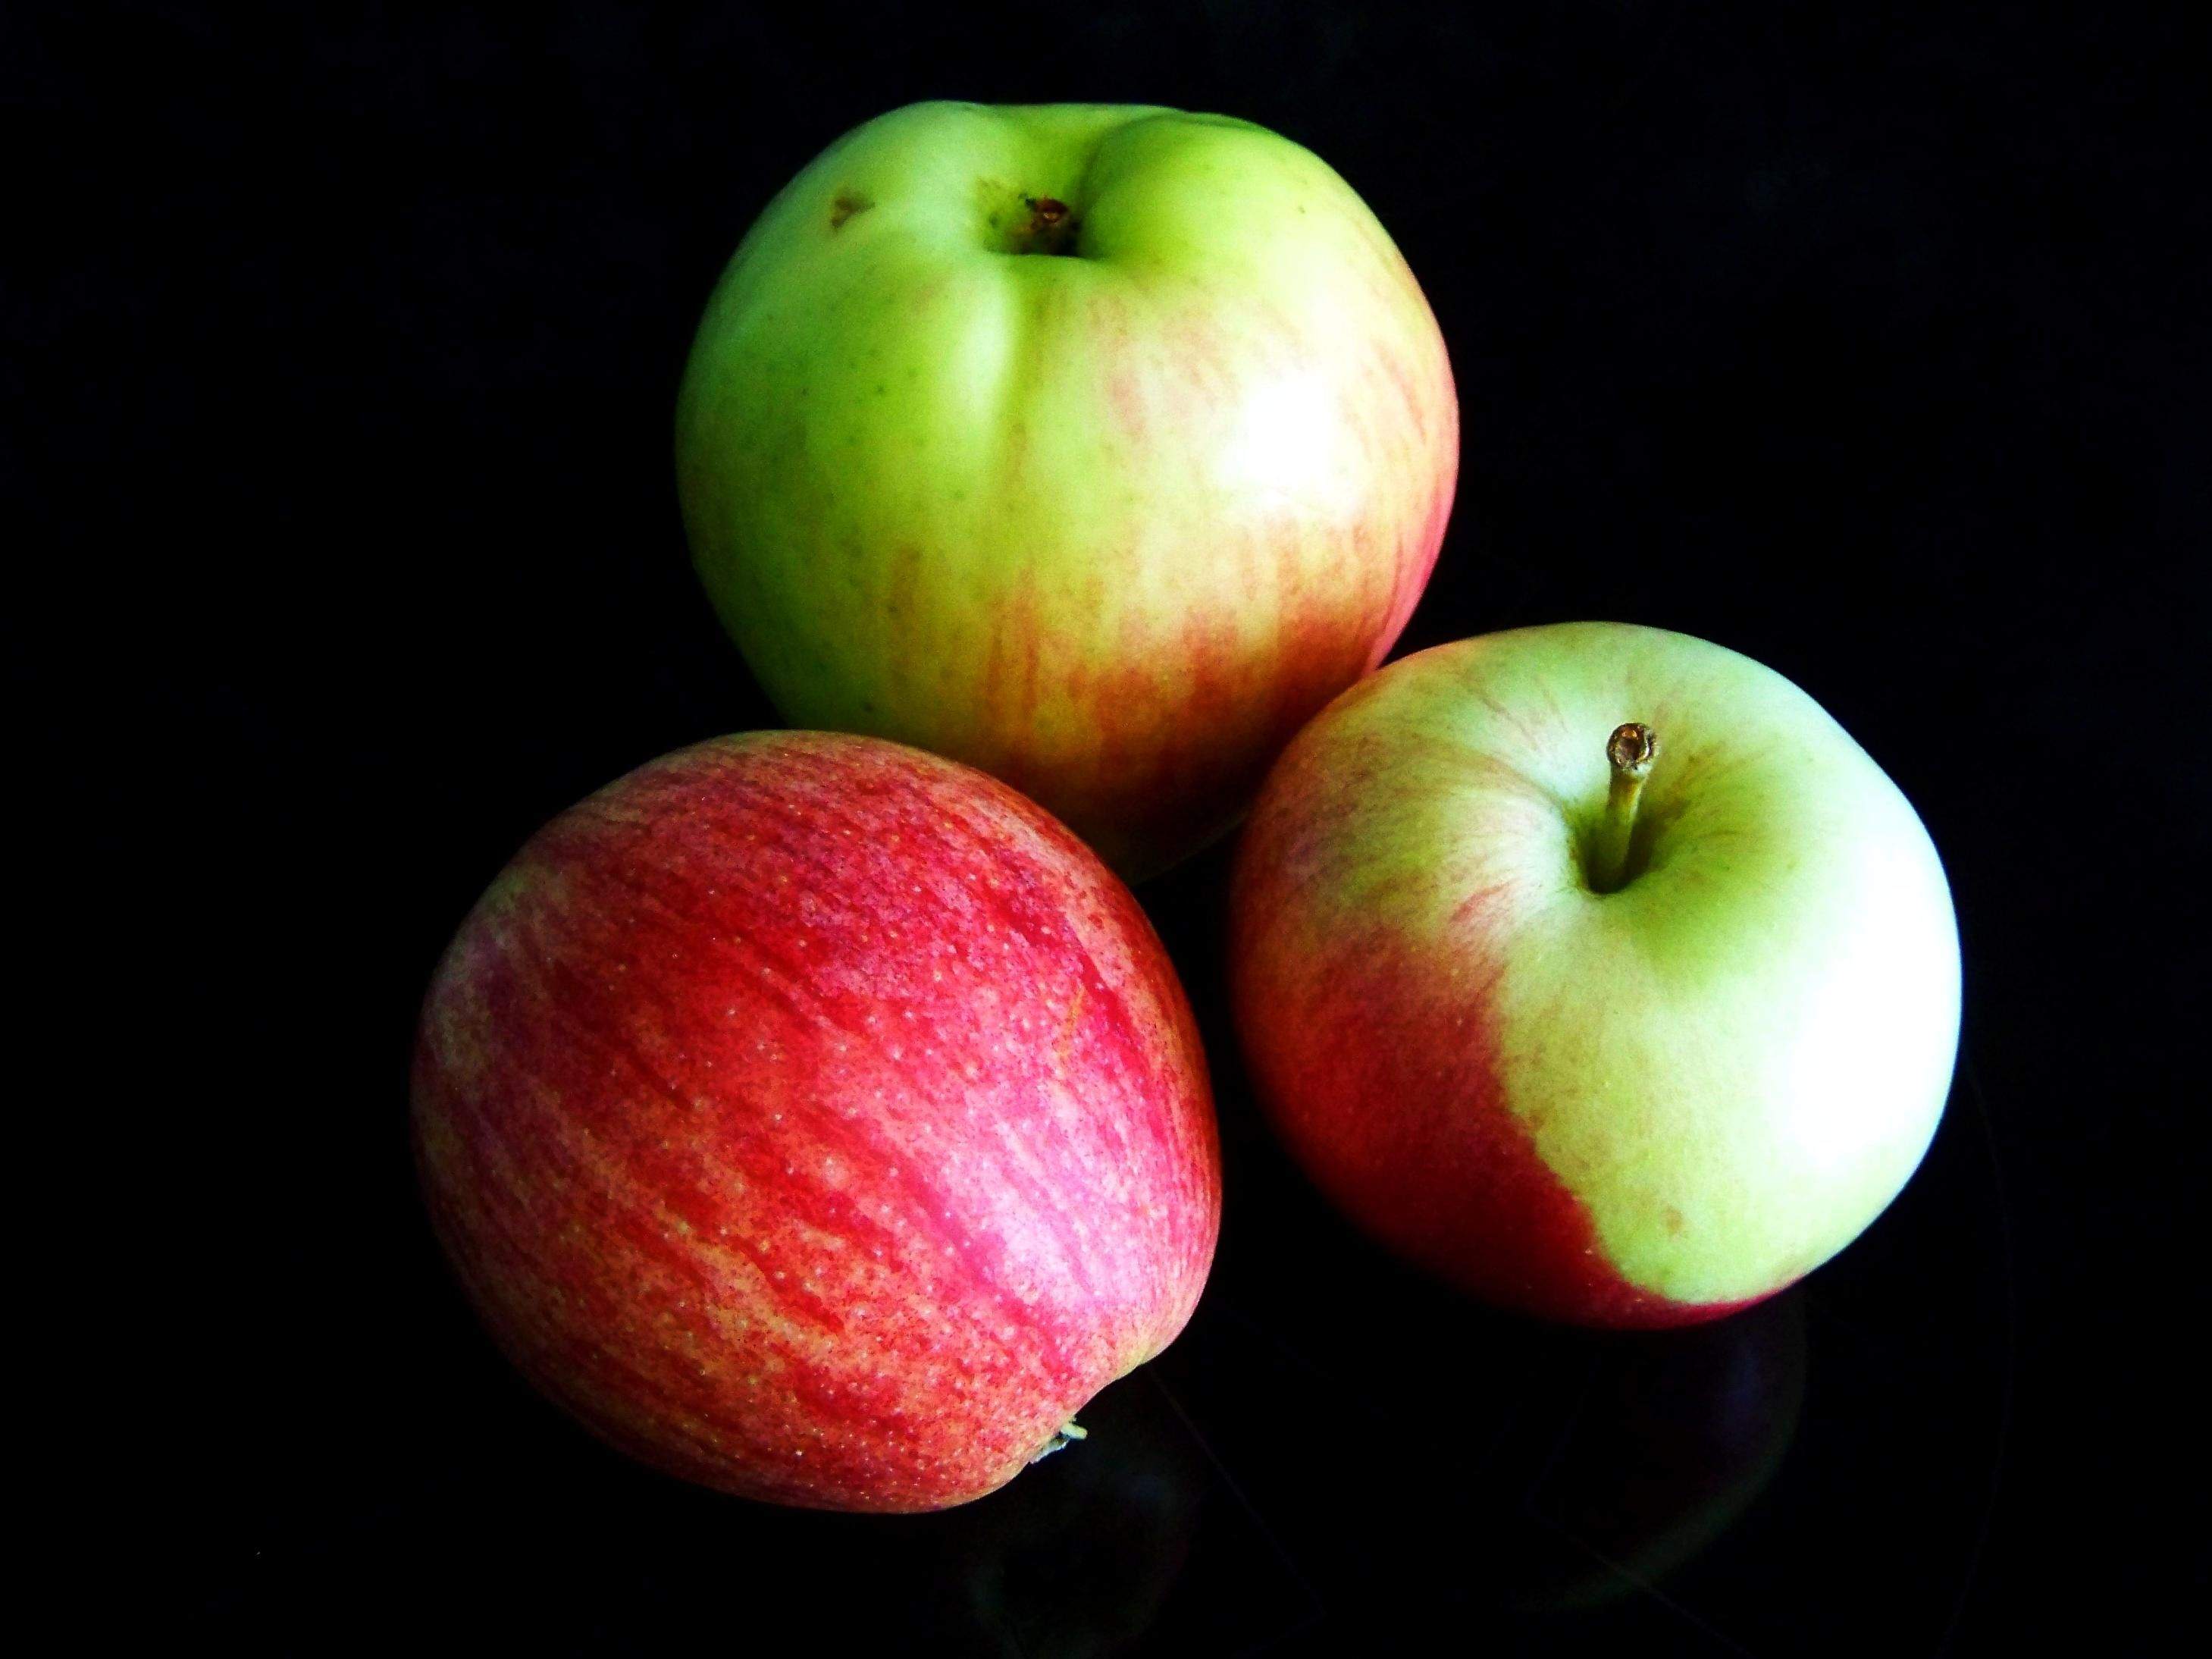
\includegraphics[width=\textwidth]{apples.jpeg}
         \caption{}
         \label{fig:apples}
     \end{subfigure}
     % \hfill
     \begin{subfigure}{0.5\textwidth}
         \centering
         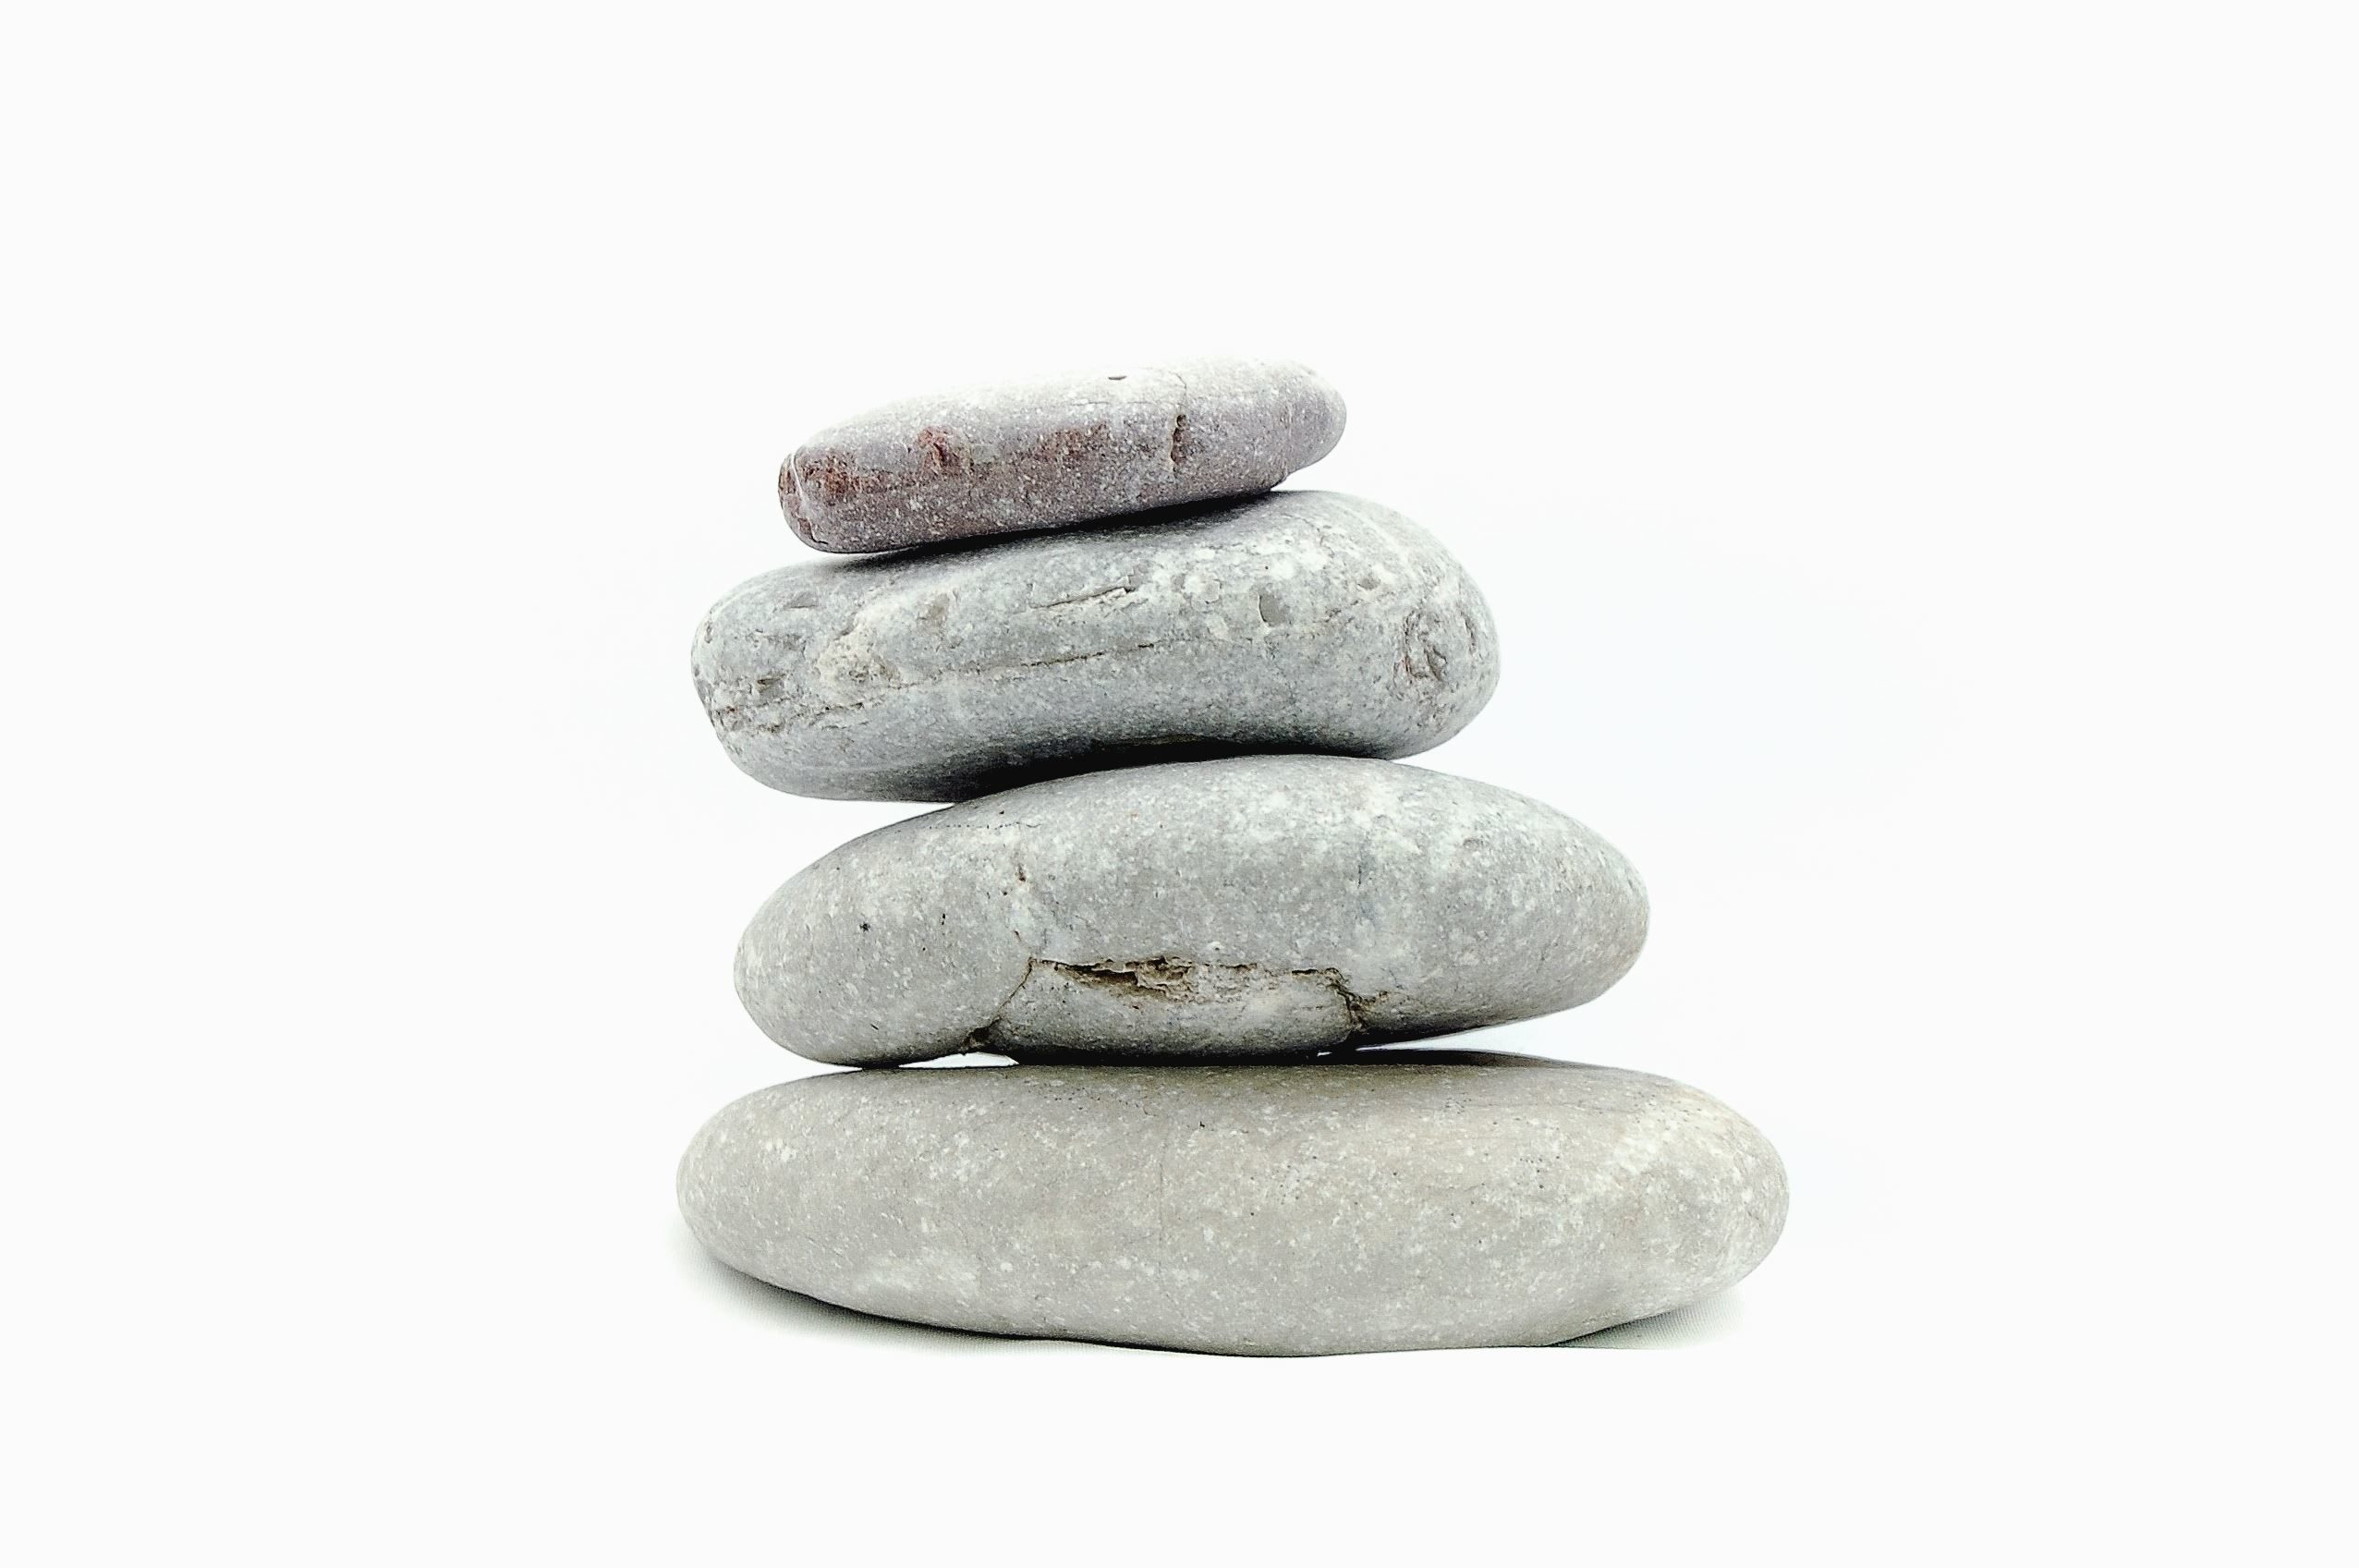
\includegraphics[width=\textwidth]{pebbles.jpeg}
         \caption{}
         \label{fig:pebbles}
     \end{subfigure}
     \caption[Correspondence between symbols and object quantities.]{(a) There are seven (7) birds in this picture, which 3 are swans and 4 are ducks. \\(b) Three (3) apples.\\ (c) Four (4) stacked pebbles.}\label{fig:exampleNumbers}
\end{figure}

%%% Local Variables:
%%% mode: latex
%%% TeX-master: "../mathematics_cheat_sheet"
%%% End:
